\chapter{Ensino, Pesquisa e Extensão}

    \section{Ensino}
    
        \begin{wrapfigure}{L}{0.3\textwidth}
            \centering
            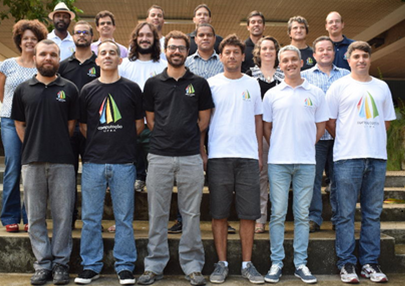
\includegraphics[width=0.29\textwidth]{ensino.png}
              \caption{Docentes - DCC/UFBA}
            \label{Rotulo}
        \end{wrapfigure}        
        Na área do Ensino a UFBA oferece cursos de Graduação e Pós Graduação em várias áreas do conhecimento, sob a orientação da Pró-Reitoria de Ensino de Graduação, órgão responsável pelo planejamento, coordenação, acompanhamento e avaliação dos cursos, onde são executadas as diretrizes de funcionamento de acordo com várias resoluções  aprovadas. Dentro da Graduação na área do Ensino o DCC oferece os seguintes Cursos:\newline
        
        
         \subsection{Graduação}
        
         \subsubsection*{Ciência da Computação}
    
    O curso de Bacharelado em Ciência da Computação da UFBA alia o estado da arte da ciência e da tecnologia da computação. Os egressos são preparados para atuar no mercado de trabalho, propondo soluções adequadas que utilizem o computador, bem como para atuar de maneira inovadora, contribuindo com o desenvolvimento tecnológico da área. Eles devem ter uma base científica que os tornem aptos a se tornarem futuros pesquisadores, de maneira a contribuir com o desenvolvimento científico da Computação. 
    
   
    \subsubsection*{Sistemas de Informação}
   O curso de Bacharelado em Sistemas de Informação da UFBA foi criado em 2010. Embora ainda seja uma área recente, já conquistou um espaço relevante no mercado de trabalho. O bacharel em Sistemas de Informação deve planejar e organizar o processamento, o armazenamento e a recuperação de informações, de modo que estas possam ser disponibilizadas aos usuários.
  
    \subsubsection*{Licenciatura em Computação}
   O curso de Licenciatura em Computação da UFBA foi criado em 2010, com o objetivo de formar profissionais de educação que atendam ao mercado de trabalho de formação básica, treinamentos e construção de conteúdos relacionados a Computação e Informática. Os egressos devem possuir uma formação sólida e abrangente de educadores, mas com base nas áreas de computação e técnicas de informática, enfatizando aspectos científicos, técnicos, pedagógicos e sociais. 
   
   
    \subsection{Pós-Graduação}
   
    \subsubsection*{Programa de Pós-Graduação em Ciência da Computação}   
    O Programa de Pós-Graduação em Ciência da Computação (PGCOMP) da Universidade Federal da Bahia (UFBA), aprovado pela CAPES, oferece os cursos de Mestrado em Ciência da Computação e de Doutorado em Ciência da Computação, com o objetivo de dar suporte à formação de pesquisadores com competência para gerar novos conhecimentos, conduzir projetos de investigação científica e exercer atividades de docência no Ensino Superior (graduação e pós-graduação lato sensu e stricto sensu) nas áreas de Ciência da Computação e Tecnologia da Informação e Comunicação (TIC).
   
    \subsubsection*{Programa de Pós-Graduação em Mecatrônica}  
    O Programa de Pós-Graduação em Mecatrônica da UFBA (PPGM), programa de pós-graduação reconhecido pela CAPES, Engenharias III, é uma iniciativa conjunta da Escola Politécnica e do Instituto de Matemática (por meio do Departamento de Ciência da Computação) da Universidade Federal da Bahia. O PPGM visa prioritariamente formar docentes, pesquisadores e engenheiros com alto nível de qualificação em sistemas mecatrônicos, de forma a ser o PPGM o locus da integração Universidade-Empresa da região, no âmbito da Mecatrônica.
    
    \subsubsection*{PRODQUAD - PROGRAMA DE QUALIFICAÇÃO DOCENTE}  
    PRODQUAD 26 11 2015.pdf, FILA DO PROQUAD APROVADA NA 86 REUNIÃO DO DCC em 20/11/2015. Esse documento foi enviado à PROPG em 26/11/2015 e os critérios permanecem os anteriores até apreciação em reunião futura do DCC.
    O quadro de docentes que compõem o  Colegiado do Curso de Ciências da Computação esta disponível em wiki.dcc.ufba.br/DCC/
    ProfessoresDcc.
    
    O quadro de docentes que compõem o  Colegiado do Curso de Ciências da Computação esta disponível em wiki.dcc.ufba.br/DCC/ProfessoresDcc.
   
    
 
    \section{Pesquisa}
   
    A maior parte da pesquisa realizada no DCC está ligada aos cursos de pós-graduação apoiados e ao 
    seu corpo docente, atuante em diversas áreas, linhas, grupos de pesquisa, que dentre outros são os seguintes:\newline
    
    \subsection{Laboratorio de Sistemas Distribuídos LaSiD}
     \begin{wrapfigure}{L}{0.3\textwidth}
            \centering
            
\includegraphics[width=0.29\textwidth]{pesquisa1.png}
        \end{wrapfigure}        
    O Laboratório de Sistemas Distribuídos ( LaSiD) é um laboratório de pesquisa dentro do Departamento de Ciência da Computação na Universidade Federal da Bahia (UFBA) . Trata-se de membros do corpo docente do Departamento de Ciência da Computação , assistentes de pesquisa e estudantes de pesquisa ( Ph.D, MSc. E Licenciatura). A missão da LaSiD é desenvolver métodos, técnicas e ferramentas que ajudam na concepção de sistemas distribuídos corretas e confiáveis, a preparar a próxima geração de pesquisadores e desenvolvedores nestas áreas por investigar problemas desafiadores.
   
    \subsection{Laboratório de Engenharia de Software LES@UFBA}
    \begin{wrapfigure}{L}{0.15\textwidth}
            \centering
            
\includegraphics[width=0.14\textwidth]{les.jpg}
        \end{wrapfigure} 
    O objetivo do Laboratório de Engenharia de Software da Universidade Federal da Bahia ( LES- UFBA) é estudar a disciplina de engenharia de software , bem como áreas que impactam a maneira como se desenvolve, mantém e gerencia software. LES tem vários grupos de pesquisa que investigam diferentes sub-áreas de engenharia de software.
    
    \subsection{Web and Interactive Systems Research Group- WISER
    (Grupo de pesquisa de Web e Sistemas interativos)}
     \begin{wrapfigure}{L}{0.3\textwidth}
            \centering
            
\includegraphics[width=0.29\textwidth]{pesquisa3.png}
        \end{wrapfigure}      
    O grupo realiza pesquisas nas áreas de Internet e Web voltadas para Web Semântica, Sistemas de Recomendação para Web, Serviços Web, Computação em Nuvem, Web e Internet das Coisas, Internet do Futuro, Recuperação da Informação na Web, Sistemas Interativos, Cidades Inteligentes e Tecnologias Assistivas. O grupo participou e participa de projetos em colaboração com outras instituições nacionais e internacionais.
     
     \subsection{Grupo de Pesquisa de Redes de Alto Desempenho- GRADE}
     \subsubsection*{OpenWiMesh:Provendo infraestrutura de comunicação sem fio como suporte à mobilidade em Smart Campi.}
      \begin{wrapfigure}{L}{0.3\textwidth}
            \centering
            
\includegraphics[width=0.29\textwidth]{pesquisa4.png}
        \end{wrapfigure}      
     Este projeto visa estudar viabilidade de implantação de uma WMN no Campus de Ondina da Universidade Federal da Bahia para ampliar o acesso a Internet dos seus usuários (alunos, professores e servidores), oferecer suporte a mobilidade de usuários móveis (usando Tablets e Smartphones) bem como oferecer QoS às aplicações educacionais que necessitam de uma infraestrutura de comunicação robusta e eficiente. 
     \subsubsection*{OpenWiMesh-MOB: Estratégias de Mobilidade em Redes Mesh Sem Fio Definidas por Software.}
    A partir do framework OpenWiMesh, este projeto visa o desenvolvimento de ferramentas e técnicas que ajudem no provimento de mobilidade transparente aos usuários móveis em uma rede mesh sem fio definida por software com a garantia de manutenção de qualidade das aplicações já acomodadas, sem necessidade de qualquer modificação nos clientes.
    
     \subsection{Inteligent Vision Research Lab
     (Laboratório de pesquisa de visão inteligente)}
     \begin{wrapfigure}{L}{0.3\textwidth}
            \centering
            
\includegraphics[width=0.29\textwidth]{pesquisa5.png}
        \end{wrapfigure} 
      As principais áreas de investigação Vision Lab estão em sistemas interactivos , detecção de objetos , imagem desempenho da classificação , compreensão cena em imagens , avaliação de classificadores de imagens , reconhecimento de ação , entre outros performance. Todas as pesquisas abrangem os campos de Cidades Inteligentes , Sistemas Inteligentes de Transporte e Sistemas biométricos.
	  
	  Um importante objetivo do laboratório é fornecer aplicações do mundo real; para isso, arquiteturas paralelas também estão sendo investigados , a fim de acelerar os sistemas propostos . Sob essa perspectiva , nós dirigimos a nossa pesquisa de requisitos acadêmicos para as necessidades da indústria , da visão a relação integrativa entre estes dois mundos.
     
     \subsection{Software Desing and Evolution Group aSide@UFBA
      (Design de Software e Grupo Evolução)}
      \begin{wrapfigure}{L}{0.3\textwidth}
            \centering
            
\includegraphics[width=0.29\textwidth]{pesquisa6.jpg}
        \end{wrapfigure} 
      O design de software requer esforço e inteligência de pessoas para a criação de artefatos de software idealmente concebidos para realizar funções úteis para pessoas. E software útil está em constante evolução. Nesse contexto, o grupo de pesquisa aSide @UFBA tem como objetivo investigar aspectos da "ciência do artificial" e de seus processos de design e evolução de software, buscando caracterizar, desenvolver e avaliar modelos, princípios, práticas e ferramentas para que pessoas possam criar, desenhar, construir, validar, reutilizar, modificar, analisar, gerenciar e desfrutar de software de qualidade. 
	  
	  O aSide @ UFBA é um grupo de pesquisa certificado pela UFBA no Diretório de Grupos do CNPq e está associado ao Laboratório de Engenharia de Software (LES) da UFBA.
     
     \subsection{Context and Ubiquitous Systems Group CEManTIKA
     (Grupo de Sistemas de Contextos)}
      \begin{wrapfigure}{L}{0.3\textwidth}
            \centering
            
\includegraphics[width=0.29\textwidth]{pesquisa7.jpg}
        \end{wrapfigure} 
     O Grupo CEManTIKA visa estudar conceitos, técnicas, modelos e ferramentas que apoiem a construção de sistemas sensíveis ao contexto. São objetivos do grupo: 
      Desenvolver sistemas sensíveis ao contexto voltados para diferentes áreas; 
      Formalizar conceitos e metamodelos para modelagem de informações de contexto; 
      Investigar algoritmos e técnicas de apoio ao processamento do contexto usando raciocínio lógico; 
      Desenvolver ferramentas de apoio ao projeto e implementação de sistemas sensíveis ao contexto. 
    
     \subsection{Formalisms and Semantic Applications Research Group FORMAS(Grupo de Pesquisa de Formalismos e \newline aplicações semânticas)}
      \begin{wrapfigure}{L}{0.3\textwidth}
            \centering
            
\includegraphics[width=0.29\textwidth]{pequisa8.jpg}
        \end{wrapfigure} 
      Objetivo principal é estudar , analisar e avaliar abordagens semânticas , cobrindo desde formalismos através de aplicações . As nossas principais áreas de investigação do grupo baseiam-se em cinco etapas principais em conseguir semântica : Métodos , ontologia, Extração de Informação , a interoperabilidade e validação formal . Lamentamos profundamente analisar cada uma dessas abordagens com foco na obtenção de altos níveis de compreensão semântica e pragmática.
    
     \subsection{Grupo de Algoritmos e Computação Distribuida Gaudi}
      \begin{wrapfigure}{L}{0.3\textwidth}
            \centering
            
\includegraphics[width=0.29\textwidth]{pesquisa9.jpg}
        \end{wrapfigure} 
     O GAUDI visa o entendimento dos problemas fundamentais que surgem na confecção de sistemas e aplicações computacionais e a busca de soluções para os mesmos. A sua principal linha de pesquisa concentra-se no estudo de algoritmos distribuídos e na sua aplicação para o desenvolvimento de componentes de software que facilitem a construção de sistemas confiáveis. 
      Linhas de Pesquisa: Algoritmos Distribuídos, Tolerância a Falhas, Componentes Distribuídos, Grades Computacionais, Redes Móveis Ad-Hoc (Manets), Teoria dos Grafos.
     
      \subsection{Formal Meethods in Software Engineering Group  MEFES
      (Métodos Formais em Grupo de Engenharia de Software)}
       \begin{wrapfigure}{L}{0.13\textwidth}
            \centering
            
\includegraphics[width=0.09\textwidth]{pesquisa10}
        \end{wrapfigure} 
      Visa a proposição de processos de desenvolvimento de softwares que sejam sistemáticos, baseados em métodos e ferramentas, e aplicáveis a sistemas reais. Tendo sempre em mente a produção de software de qualidade, dentro de limites previsíveis de tempo e custo.
    
      \subsection{Reuse in Software Engineering Group RiSE
      (Grupo de Engenharia de Software-reutilizacao)}
       \begin{wrapfigure}{L}{0.3\textwidth}
            \centering
            \includegraphics[width=0.29\textwidth]{pesquisa11}
        \end{wrapfigure} 
      O objetivo deste projeto é investigar e definir um processo para o desenvolvimento de linhas de produtos orientadas a serviços . O processo proposto envolve as fases de definição de escopo , requisitos e design. Definir um programa de reutilização de software para educar engenheiros de software high- especializados centrados em princípios de reutilização e ideias.
    
     \subsection{Software Visualization Group SoftVis
      (Grupo de vizualizacao de software)}
      O grupo tem como objetivo desenvolver metodologias , ferramentas e técnicas para visualização de software ( SoftVis ) e empiricamente caracterizar e avaliá-los. Tem o interesse especial no desenvolvimento de ambientes SoftVis que podem ser integrados para IDEs para reforçar atividades de compreensão de software e ajudar em tarefas de engenharia de software . Com esse objetivo , temos desenvolvido vários projetos.
     
     \subsection{Sistemas de Tempo Real}
      Grupo de pesquisa focada no desenvolvimento de novas técnicas para a concepção, análise e implementação de sistemas de tempo real. O nosso grupo foi oficialmente certificada pela UFBA em maio de 2014. A nossa equipa tem vindo a investigar vários aspectos dos sistemas em tempo real , com especial ênfase no multiprocessador / multicore escalonamento de tempo real.
     
     \subsection{ONDA DIGITAL - Grupo de Pesquisa e Extensão em Informática, Educação e Sociedade.}
      Grupo de Pesquisa e Extensão em Informática, Educação e Sociedade tem como eixo integrador as relações interdisciplinares entre Computação, Educação e Sociedade com especial interesse nas seguintes áreas: 
      
      (1) informática na educação; 
      
      (2) interação humano-computador (teoria, desenvolvimento e avaliação de tecnologias interativas); 
      
      (3) educação em computação; 
      
      (4) informática, educação e sociedade. Desde 2004 o grupo tem estabelecido parcerias com a indústria de software, instituições educacionais e outros parceiros financiadores de projetos. Mais de 100 estudantes de graduação passaram pelo grupo ao longo dos últimos dez anos. Atualmente temos mais de 40 alunos, entre pesquisadores, estudantes de graduação, mestrado e doutorado.
     
      \subsection{Computational Intelligence and Optimization Research Lab
      (Laboratorio de Pesquisa em Inteligência Computacional e Optimização)}
     Inteligência Computacional é uma das áreas de Inteligência Artificial que lida com a aquisição de conhecimento automático. O nosso grupo está focado na teoria , aplicação e desenvolvimento de métodos de inteligência computacional .
	  
	  Optimização é uma das áreas de pesquisa operacional que lida com a encontrar as melhores soluções possíveis para os problemas . Nosso trabalho concentra-se na elaboração de teoria, modelos e algoritmos para problemas de optimização.
	  
	  Pesquisa em Sistemas Computacionais lida com os sistemas de software / hardware distribuídos concepção e avaliação de paralelo complexo e . Nosso grupo tem foco especial na alocação inteligente dos recursos de computação destinados a reduzir o consumo de energia / energia com garantias de desempenho em tempo real.
	  
      Todas as informacões sobre os grupos de pesquisa estao disponiveis em wiki.dcc.ufba.br/DCC/GruposDePesquisa.
    
     
      
      \section{Extensão}
      
     O DCC oferece atualmente três atividades permanentes de extensão -- o Programa Onda Digital, o Programa de Ações Pedagógicas para Formação de Professores de Computação (PROFCOMP) e a Especialização Avançada em Sistemas Distribuídos. Além dessas atividades, executamos outras ações eventuais e sob demanda, inclusive cursos de extensão para organizações públicas e privadas. 
      
      Ao longo dos anos, docentes do DCC tem organizado eventos regionais, nacionais e internacionais, e participado de projetos de extensão voltados para a sociedade baiana. 
      
      Para obter maiores informações sobre os cursos ou outras atividades de extensão, envie uma mensagem para a Profa. Debora Abdalla, coordenadora de Atividades de Extensão do DCC. 
    
       \subsection{Programa Onda Digital}
      O Onda Digital é um programa de Extensão permanente e visa a participação ativa da universidade dentro da comunidade em prol da inclusão digital. O Programa abrange ações educativas, de desenvolvimento de recursos humanos e técnicos e de criação e uso de software livre voltados para viabilização e melhoria dos processos de inclusão digital. Informações em wiki.dcc.ufba.br/bin/view/
       OndaDigital
      
       Atividades do Programa: 
       
       
       \subsubsection*{Criação do Grupo Colméia} 
       O Colméia tem por objetivo de disseminar o conhecimento digital, sem fronteiras sociais e sem barreiras culturais. O grupo é formado por professores do DCC, alunos voluntários do curso de computação com apoio da InfoJr, DACOMP, pessoas do CPD-UFBA e membros do PSL-BA. O grupo atuou no convênio com a ONG Eletro cooperativa e ministrou um curso de Iniciação a Informática para jovens.
       
       \subsubsection*{Oficina Teoria e prática educacional em projetos de inclusão digital}
       
       Esta oficina visa preparar instrutores de cursos de inclusão digital no planejamento, execução e avaliação desses cursos. A oficina aborda, de forma teórico-prática, aspectos didáticos e pedagógicos que influenciam o sucesso de cursos voltados para a inclusão digital. A oficina terá duração de 12 horas.  
     
     \subsection{Programa de Ações Pedagógicas para Formação de Professores de Computação (PROFCOMP)}
    O PROFCOMP é um programa de Extensão permanente que integra ações educativas voltadas à inserção escolar do licenciando em computação como elemento mediatizador de ações pedagógicas interdisciplinares com uso de tecnologias digitais e do pensamento computacional com e sem uso de computadores. As ações do programa contam com apoio da Pró-Reitoria de Extensão da UFBA e pretendem contribuir à formação de professores e estudantes para a efetiva apropriação da "cultura digital" nas escolas. 
      
      \subsection{Especialização Avançada em Sistemas Distribuídos(latu sensu)}
      
      
     A Especialização Avançada em Sistemas Distribuidos é um programa lato sensu em que as áreas de concentração foram escolhidas de forma a complementar as demandas mais freqüentes de profissionais em nossa região e segundo as áreas de competência dos professores do Departamento de Ciência da Computação e do Laboratório de Sistemas Distribuídos.  Informações em lasid.ufba.br/easd/especializacao.html. 
      
      \subsection{Grupo de Programação (grupro)}
      
      É um grupo de professores e alunos com vários interesses interligados, sendo o principal deles a participação em maratonas de programação. O grupro busca melhorar a qualidade dos cursos de graduação através da inserção da cultura de maratonas de programação no dia a dia das disciplinas de computação, aprimorar o perfil dos alunos egressos, e dar visibilidade a estes alunos através de bons desempenhos em competições relacionadas. Além disso, busca uma atuação mais representativa da cidade de Salvador e do estado da Bahia em competições nacionais e internacionais de programação. Informações em http://maratona.dcc.ufba.br. 
      
